\documentclass[12pt]{exam}
\usepackage[utf8]{inputenc}

\usepackage[margin=1in]{geometry}
\usepackage{amsmath,amssymb}
\usepackage{multicol}
\usepackage{amsmath}
\usepackage{fullpage}
\usepackage{graphicx}



\usepackage{tikz}
\usetikzlibrary{plotmarks, chains}
\usetikzlibrary{fit,positioning,arrows,automata}

\newcommand{\class}{ML \& Statistics I}
\newcommand{\term}{Winter 2017}
\newcommand{\examnum}{Exam 1}
\newcommand{\examdate}{09-Nov-2017}
\newcommand{\timelimit}{45 Minutes}

\pagestyle{head}
\firstpageheader{}{}{}
\runningheader{\class}{\examnum\ - Page \thepage\ of \numpages}{\examdate}
\runningheadrule


\begin{document}

\noindent
\begin{tabular*}{\textwidth}{l @{\extracolsep{\fill}} r @{\extracolsep{6pt}} l}
\textbf{\class} & \textbf{Name:} & \makebox[2in]{\hrulefill}\\
\textbf{\term} &&\\
\textbf{\examnum} &&\\
\textbf{\examdate} &&\\
\textbf{Time Limit: \timelimit} & Teaching Assistant & \makebox[2in]{\hrulefill}
\end{tabular*}\\
\rule[2ex]{\textwidth}{2pt}

This exam contains \numpages\ pages (including this cover page) and \numquestions\ questions.\\
Total of points is \numpoints.

This test is to design the course. A similar level test will be designed after the course. Rest of introduction. Rest of introduction. Rest of introduction. Rest of introduction. Rest of introduction. All the best. 


\begin{center}
Grade Table (for coordinator's use only)\\
\addpoints
\gradetable[v][questions]
\end{center}

\noindent
\rule[2ex]{\textwidth}{2pt}
%*******************************************************
%*******************************************************
%*******************************************************
\begin{questions}

\question[3] You are working on a particular learning task and cross-validation experiments indicate that your SVM is overfitting. Name three action that can help decrease overfitting in an SVM.
\makeemptybox{2in}
\addpoints
%*******************************************************
%*******************************************************

%*******************************************************
%*******************************************************
\question[4] You have an application problem for which you need to decide whether to use a Two-Layer Neural Net or Support Vector Machine with a non-linear kernel. What would be your arguments in favor of the Net, and arguments in favor of SVM.
\makeemptybox{3in}
%*******************************************************
%*******************************************************
\question[1] In the multiple linear regression model, the adjusted $R^2, \overline R^2 $ : \\
\begin{oneparchoices}
\choice cannot be negative \\
\choice will never be greater that the regression $R^2$ \\
\choice equals the square of the correlation coefficient r \\
\choice cannot decrease when an additional explanatory variable is added \\
\end{oneparchoices}
%*******************************************************
%*******************************************************
\question[2] The following linear hypothesis can be tested using the $F$-test with the exception of \\
\begin{oneparchoices}
\choice $\beta_2$ and $\beta_3 =  \frac{\beta_4}{\beta_5}$ \\
\choice $\beta_2 = 0$ \\
\choice $\beta_1 + \beta_2 =  1$ and $\beta_3 = -2 \beta_4$ \\
\choice $\beta_0 = \beta_1$ and $\beta_1 = 0$ \\
\end{oneparchoices}
%*******************************************************
%*******************************************************
\question[12] Mark box if true.
\addpoints
\begin{checkboxes}
\choice AdaBoost will eventually reach zero training error, regardless of the type of weak classifier it uses, provided enough weak classifiers have been combined. % False! If the data is not separable by a linear combination of the weak classifiers, AdaBoost can’t achieve zero training error. 
\choice If the outcome variable is quantitative and all explanatory variables take value 0 or 1, a logistic regression model is most appropriate. % False. Logistic regression is only appropriate when the outcome variable is 0/1.
\choice Cross validation will guarantee that our model will not overfit. % False
\choice Logistic regression is a supervised machine learning algorithm % True
\choice To analyze the performance of Logistic Regression, we use AIC. We prefer a model with minimum AIC value. % True
\choice Standardization of features is required before training a Logistic Regression % False
\choice Both LASSO and Ridge is used for variable selection % False, only LASSO is used
\choice probability density function's value can be greater than 1
\choice Exponential Distribution and Chi Square distribution are special cases of Gamma distribution
\choice Student's t-distribution has a thicker ($\geq$) tail than Standardized Normal distribution
\choice Uniform distribution is a discrete distribution
\choice In PCA, the first princial component, is given by the linear combination of the original variables with the minimum possible variance
\choice Learning the parameters for a neural network is a convex optimization problem. % FALSE. It is non-convex. Easy to get, stuck in a local minima. Learning for logistic regression is a convex optimization problem. We can always find the globally optimal solution. 
\choice KNN handles non-linearly separable classes much better than logistic regression % TRUE
\end{checkboxes}



{%
% changing choice items style locally
\renewcommand*\thechoice{\arabic{choice}} 
\renewcommand*\choicelabel{\thechoice)}
%
%*******************************************************
%*******************************************************
\question[1] Given the following data samples (square and triangle mean two classes), which one(s) of the following kernels can we use in SVM to separate the two classes \\
\begin{figure}[h]
\centering
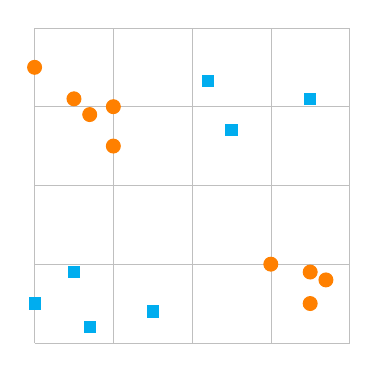
\begin{tikzpicture}
\draw [very thin, lightgray] (0,0) grid (4,4);
\draw [cyan] plot [only marks, mark=square*] coordinates {(3.5,3.1) (2.2,3.33) (2.5,2.7) (0,0.5) (0.5,0.9)(0.7,0.2)(1.5,0.4)};
\draw [orange] plot [only marks, mark size=2.5, mark=*] coordinates {(0,3.5) (0.5,3.1) (0.7,2.9) (1,2.5) (1,3.0) (3,1) (3.5,0.9)(3.7,0.8)(3.5,0.5)};
\end{tikzpicture}
\caption{SVM Kernels}
\end{figure}
\begin{multicols}{2}
\begin{choices}
\choice Linear kernel % False
\choice Polynomial kernel % True
\choice Gaussian RBF (radial basis function) kernel % True
\choice None of the above % False
\end{choices}
\end{multicols}
}%

%*******************************************************
%*******************************************************
{%
% changing choice items style locally
\renewcommand*\thechoice{\arabic{choice}} 
\renewcommand*\choicelabel{\thechoice)}
%
\question[1] The parameters to be estimated in the simple linear regression model $Y = \alpha + \beta x + \epsilon \quad \epsilon \sim N(0,\sigma)$ are :\\
\begin{multicols}{2}
\begin{choices}
\choice $\alpha , \beta, \sigma$
\choice $\alpha , \beta, \epsilon$
\choice $a , b, s$
\choice $\epsilon , 0, \sigma$
\end{choices}
\end{multicols}
}%
%*******************************************************
%*********************************************
\question[5]
In the context of classification, explain the ROC Curve \& Confusion matrix.
\makeemptybox{3in}
%*******************************************************
%*********************************************
\question[5] Suppose you want to build a decision tree for a problem. In the dataset, there are two classes with 150 examples in the + class and 50 examples in the - class.\\
Recall the definitions of information gain and entropy:
\begin{align*}
Entropy(C) &= H(C) = \sum_c - P(C=c)log_2P(C=c) \\
Gain(C,A) &= H(C) - \sum_{v \in Values(A)} P(A=v) H(C|A=v)
\end{align*}
What is the entropy of the class variable (you can leave this in terms of logs)
\makeemptybox{1.5in}

\addpoints
%*******************************************************
%*******************************************************
\question[5]
How does classification differ from clustering? \\
Explain the difference between K-nearest neighbor classification \& k-means clustering in terms of their algorithm steps.
\makeemptybox{3in}
%*******************************************************
%*******************************************************
\question[3]Consider a Markov chain whose transition diagram is as given. 
\noaddpoints % to omit double points count
\begin{parts}
\part[1] Which (if any) states are absorbing?
\part[1] Find the communicating classes.
\part[1] Is the chain irreducible?
\end{parts}
\addpoints
\begin{figure}[!h]
\centering
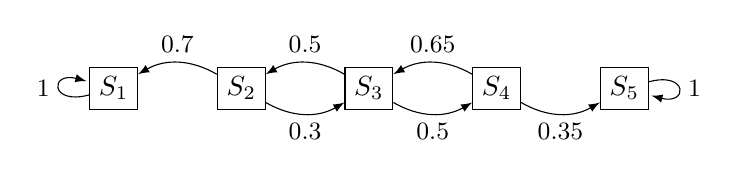
\begin{tikzpicture}[
mynode/.style={
  draw,
  minimum size=1em
  },
every loop/.append style={-latex},  
start chain=going right  
]
\foreach \Value in {1,...,5}
  \node[mynode,on chain] (s\Value) {$S_{\Value}$};
\path[-latex]
  (s2) edge[bend right] node[auto,swap,font=\small] {$0.7$} (s1)
  (s2) edge[bend right] node[auto,swap,font=\small] {$0.3$} (s3)
  (s3) edge[bend right] node[auto,swap,font=\small] {$0.5$} (s2)
  (s3) edge[bend right] node[auto,swap,font=\small] {$0.5$} (s4)
  (s4) edge[bend right] node[auto,swap,font=\small] {$0.65$} (s3)
  (s4) edge[bend right] node[auto,swap,font=\small] {$0.35$} (s5)
  (s1) edge[loop left] node[left,font=\small] {$1$} (s1)
  (s5) edge[loop right] node[right,font=\small] {$1$} (s5);
\end{tikzpicture}
\caption{Markov Chain}
\end{figure}
%*******************************************************
%*********************************************
\question[4]
Explain strong stationarity \& weak stationarity
\makeemptybox{\fill}
%*******************************************************
%*********************************************
\question[4]
How is $p, q$ decided in $ARMA(p,q)$ model? 
\makeemptybox{\fill}
%\newpage
%*******************************************************
%*******************************************************
\question[5]
Ridge Regression, Lasso Regression, and Elastic Net are used to implement three different ways to constrain the weights to achieve regularization for a linear model. What are those ways?
\fillwithlines{\fill}

%\newpage
%*******************************************************
%*******************************************************
\question[5]
The \textit{perceptron} is one of the simplest Artificial Neural Network architecture. Explain the algorithm and how it works.

\fillwithdottedlines{8em}
%*******************************************************
%*******************************************************
\question[6] Consider the following HMM: 
\begin{figure}[!htb]
\begin{tikzpicture}
\clip (-2.5,-2.5) rectangle (8.5,2.5);
\tikzstyle{main}=[circle, minimum size = 5mm, thick, draw =black!80, node distance = 10mm]
\tikzstyle{connect}=[-latex, thick]
\tikzstyle{box}=[rectangle, draw=black!100]
  \node[box,draw=white!100] (Latent) {\textbf{Latent}};
  \node[main] (L1) [right=of Latent] {$X_1$};
  \node[main] (L2) [right=of L1] {$X_2$};
  %\node[main] (L3) [right=of L2] ;
  %\node[main] (Lt) [right=of L3] ;
  \node[box,draw=white!100] (Observed) [below=of Latent] {\textbf{Observed}};
    \node[main,fill=black!10] (O1) [right=of Observed,below=of L1] {$O_1$};
  \node[main,fill=black!10] (O2) [right=of O1,below=of L2] {$O_2$};
 % \node[main,fill=black!10] (O3) [right=of O2,below=of L3] {$O_3$};
  %\node[main,fill=black!10] (Ot) [right=of O3,below=of Lt] {$O_t$};
  \path (L3) -- node[auto=false]{\ldots} (Lt);
  \path (L1) edge [connect] (L2) ;
        %(L2) edge [connect] (L3)
        %(L3) -- node[auto=false]{\ldots} (Lt);
  %\path (O1) edge [connect] (O2) ;
        %(O2) edge [connect] (O3)
        %(O3) -- node[auto=false]{\ldots} (Ot);
  \path (L1) edge [connect] (O1);
  \path (L2) edge [connect] (O2);
  %\path (L3) edge [connect] (O3);
  %\path (Lt) edge [connect] (Ot);
  \draw[dashed]  [below=of L1,above=of O1];

\path (Latent) -- (Observed) coordinate[midway](l44);
\node (l43) [left=of l44] {};
%\path (Lt) -- (Ot) coordinate[midway](l444);
\node (l433) [right=of l444] {};
\draw[dashed,thick] (l43) to ++(0:150);

\end{tikzpicture}
\end{figure}





\begin{table}[!htb]
    \caption{HMM}
    \begin{minipage}{.2\linewidth}
      \caption{}
      \centering
        \begin{tabular}{ |c|c| } 
 \hline
 $X_1$ & $P(X_1)$  \\ 
 \hline
 0 & 0.3  \\ 
 1 & 0.7  \\ 
 \hline
\end{tabular}
    \end{minipage}%
     \begin{minipage}{.4\linewidth}
      \centering
        \caption{}
        \begin{tabular}{ |c|c|c| } 
 \hline
 $X_t$ & $P(X_{t+1})$ &  $P(X_{t+1}|X_t)$\\ 
 \hline
 0 & 0 & 0.4  \\ 
 0 & 1 & 0.6  \\ 
 \hline
 1 & 0 & 0.8  \\ 
 1 & 1 & 0.2  \\
 \hline
\end{tabular}
    \end{minipage}
    \begin{minipage}{.4\linewidth}
      \centering
        \caption{}
        \begin{tabular}{ |c|c|c| } 
 \hline
 $X_t$ & $P(X_{t+1})$ &  $P(X_{t+1}|X_t)$\\ 
 \hline
 0 & A & 0.9  \\ 
 0 & B & 0.1  \\ 
 \hline
 1 & A & 0.5  \\ 
 1 & B & 0.5  \\
 \hline
\end{tabular}
    \end{minipage} 
\end{table}
\noaddpoints % to omit double points count
\begin{parts}
\part[3] Use the forward algorithm to compute the probability distribution $P(X_2, O_1 = A, O_2 = B)$. Show your work. You do not need to evaluate arithmetic expressions.
\makeemptybox{1.5in}
\part[3] Compute the probability distribution $P(X_1 = 1| O_1 = A, O_2 = B)$. Show your work.
\makeemptybox{1.5in}
\end{parts} 

\addpoints
%*******************************************************
%*******************************************************
\question[4]
Explain the following equation (in terms of multivariate linear regression):\\
\begin{equation}
\hat{\beta} = (X^TX)^{-1}X^TY
\end{equation}
Give numbers for the dimensions of the matrix as well
\makeemptybox{3in}
%*******************************************************
%*******************************************************
\end{questions}

\end{document}
